\section{Detectors [Ilhan, Laurent]}
\label{sec:detectors}

In this white paper, all technologies assumed in the definition of the detectors design are chosen through their maturity for integration.
Thus, none of the sub-detectors proposed require a major R\&D effort threatening the implementation of the LHeC/\lhuc detector concepts discussed here.

\subsection{LHeC}
\label{subsec:detLHeC}

\subsubsection{Flagship design: 50--60 GeV electron beams}

The main design choices for the LHeC detector concept are described in \cite{LHeCStudyGroup:2012zhm,LHeC:2020van,Ahmadova:2025vzd}.
From the interaction region outwards, and as depicted in Fig.\,\ref{fig:lhec_detector_concept}, a longitudinally asymmetric tracker surrounds the interaction point.
It relies on existing CMOS technologies, with a central barrel composed of 4 layers of pixels and 5 layers of macro-pixels, 2 wheels in the central endcaps, and 3 and 5 wheels in the backward (following the electron direction), and forward (hadron direction) endcaps respectively.

Consecutive to the tracker component, both a barrel and end caps section of an electromagnetic, and a hadronic calorimeters are located outside the volume of an inner superconducting 3.5~T solenoid.
For the barrel section, the proposed design for the electromagnetic part is a liquid argon calorimeter ($28-30X_0$) with an ATLAS-like accordion structure, and a hadronic part composed of iron absorbers adding up to an interaction length $\sim8-12\lambda_I$.

Finally, at the outermost section of the LHeC detector, an array of muon detectors is placed with gas chambers technologies already successfully operating in the (HL-)LHC environment: resistive plate chambers, cathode strip chambers, and others.

\begin{figure}
\centering
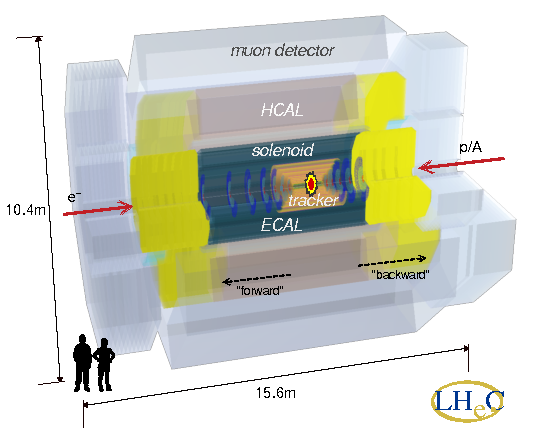
\includegraphics[width=.8\textwidth]{lhec_detector_annotated_nobackground.pdf}
\caption{Cutaway drawing of the LHeC detector concept as described in the CDR, and bridge concept papers.}
\label{fig:lhec_detector_concept}
\end{figure}

\add{[synchrotron radiation study]}

Outside the interaction region, a circular-elliptic geometry for the beamline is optimised to fit the dynamics of a three-beam system.
Furthermore, it allows an efficient fanning of the synchrotron radiation emitted by the lepton bending close to the interaction point.

While a detailed simulation of all detector components described in this section is required for the optimisation of key operational parameters, this goes beyond the scope of this proposal.
Both a DELPHES 3 detector description of all appartuses, and a Key4hep stack are however under construction, and will be described in a follow-up publication.

\subsubsection{Staged design: 20 GeV electron beams}

In the case of a staged configuration as described in \cite{Andre:2025iar}, a lower energy baseline may be defined as a first step in the construction of the nominal LHeC.
Based on a single-pass acceleration through the two 10-GeV linacs, the 20 GeV electron beam configuration induces an additional boost of the central system in the direction of the proton.
Therefore, a modified design covering an extended rapidity acceptance is required to ensure a good reconstruction of flagship DIS, $t\bar t$, and Higgs final states.
This includes calorimetry up to $\eta\sim$ \add{xxx}, and good tracking performances at a shorter distance to the beams, thus in a challenging radiation environment, especially in the very forward region.

The centre-of-mass energy for electron-hadron being reduced from $1.2$ to $0.75$ TeV in this operational mode, the radiative power emitted mainly by synchrotron radiation, is also reduced by a factor \add{XXX}, thus diminishing the need for additional shielding of the critical proton focussing/defocussing quadrupoles in the vicinity of the electron bending magnets.
This allows a relaxed design of the very forward region of the detector acceptance, and the possibility of an increased segmentation in this region of interest.

\subsubsection{Forward proton detectors}

Specific physics cases (e.g. involving the exchange of a colour-singlet such as photons, or pomerons, \ldots) allow high-energy interactions to occur in the vicinity of the lepton-hadron collision point without the fragmentation of the scattered proton after the exchange.
Referred to as central exclusive processes (CEP), these provide a laboratory for low-rate, high-precision searches described in section \ref{paragraph:twophoton}.
Instrumentation of the forward near-beam region is crucial for the direct tagging of this particular class of events where a proton is detected, and to precisely determine the scattered muons momentum to ensure a good reconstruction of the the DIS kinematic variables.
Multiple technologies have already demonstrated their ability to observe the scattered protons a few units of the beam separation $\sigma_{x,y}$ in a radiation-hard environment: so-called Roman Pots \cite{CMS:2024xbs,ATLAS:2024ztz}, or moveable (Hamburg) beam pipes.
Both the proton, and the lepton spectrometer systems may therefore consist of heterogeneous detectors composed of layers of silicon-based tracking detectors, such as the ones of the CMS Precision Proton Spectrometer \cite{CMS:2014sdw} and its HL-LHC upgrade \cite{CMS:2021ncv}.

%in the far forward direction and a muon system in the far backward direction mounted on the beam pipe outside the detector able to measure muons with reasonable resolution down to very small scattering angles and at momenta up to the beam to detect the scattered protons and muons, respectively.


\subsection{\texorpdfstring{LH$\mu$C}{LHuC}}
\label{subsec:detLHuC}

Recently, general-purpose detector design studies have been presented for the detection of particles produced by muon-hadron collisions\cite{Acosta:2023,Akturk:2025ubm}. The detector structure given in these studies is configured superconducting solenoid magnet for precise momentum measurements for charged tracks. It consists of a silicon tracker to provide precision timing and position information, a particle identification system located outside of the silicon tracker, electromagnetic and hadronic calorimeters to precisely measure the energies of the particles, and muon spectrometer to measure muons with proper resolution. These sub-detectors surround the beam pipe. On the beam pipe outside the detector, Roman Pots in the far forward direction and a Muon System in the far backward direction are mounted to detect the scattered protons and muons, respectively. 

Beam induced backgrounds are one of the main challenges in designing the muon collider detectors. The case for muon-hadron collision requires the consideration of shielding of critical elements following the direction of the muon beam. This latter, with a flux estimated at high values in the design luminosity considered here, is expected to deliver an intense source of secondary radiation through ionisation and bremsstrahlung emissions. In order to protect the innermost detector elements, a tungsten nozzle shielding cladded with borated polyethylene is placed on the coming muon side.

The studies on dedicated detector design will be performed corresponding to the acceptance, resolution, and calibration goals which arise from the muon-hadron collision physics programs. The realistic dimensions of the detector and its sub-components will be determined using detailed GEANT4 and FLUKA simulations to get the detector's response to particles generated from the collision. Shielding studies will be detailed to optimize the overall physical performance of the detector. The variations of the energy depositions at different muon energies traversing such a cone made of different stopping target materials will be studied. 


\subsubsection{Physics motivated requirements}

In order to translate the kinematic requirements defined for the LHeC/\lhuc physics case described in Section\,\ref{sec:physics} into constraints on acceptance and rates estimates, a {DELPHES} 3 \cite{deFavereau:2013fsa} modeling of the detector concept is defined. During modeling, the physical requirements mentioned below should also be considered based on the geometry defined for the LHeC CDR studies.


As the baseline \lhuc described here proposes the collision of a 7 TeV proton beam against a 1 TeV muon beam, the instrumentation of the detector is asymmetric, following the asymmetric nature of the collisions.
The physics program of the muon-hadron collision motivates strict demands for detector such as hermetic coverage, strong forward and backward acceptance, precision tracking, a finely segmented calorimetry system, and a good shielding from beam induced background. 

Following the physics case described in Section \ref{sec:physics}, the production of BSM particle decaying to missing energy final states imposes detector hermeticity for missing energy signatures.
In terms of the DIS kinematics, the proton structure is precisely examined over an extended Bjorken-x and $Q^2$ phase space. This strongly motivates excellent forward and backward acceptance, precise measurement of the small-angle scattered lepton and hadronic final state.

A major source of the beam induced background is the decay of primary muons and the interaction of their decay products with the beam pipe.
In order to prevent the decay products from entering the detector, the muon beam line should be coated with a tungsten nozzle. The nozzle is coated with borated polyethylene to reduce the amount of neutrons produced from interactions within the tungsten core. The occupancy in the tracking system could be improved with the optimized nozzle.

For the precision of the electroweak and QCD measurements, high-resolution central tracking and finely segmented electromagnetic calorimetry should be used. A silicon tracker system with precision timing information is critical for performing meaningful physics analyzes. It would have 4-D tracking using Low Gain Avalanche Diodes (LGADs) or  PICOSEC-Micromegas (PICOSEC-MM) \cite{Malberti:2026}. The particle identification system is crucial for QCD measurements. Maintaining a very high tracker occupancy under beam-induced background conditions is an essential performance factor.

\subsubsection{\texorpdfstring{$\mu^+$}{Muon} shielding}

With a fraction of the muons decaying despite their acceleration in the relativistic regime, a large amount of background particles such as photons, electrons and neutrons are expected in the vicinity of the interaction region.
These particles are foreseen to generate visible signals in the detector, undistinguishable from the muon-hadron collisions.
The effect of beam-induced background depends on the energy of the muon beam, machine optics, and lattice elements.
According to previous studies~\cite{Collamati:2021,Bell:2025}, massive reductions of beam induced backgrounds can be obtained by means of a careful optimization of the Machine Detector Interface (MDI) and timing selection.
A conical tungsten nozzle cladded with borated polyethylene, placed around the muon beam line near the interaction point, is also used as the primary beam induced backgrounds mitigation element.
Its main purpose is to block the muon decay products before they enter the sensitive detector volume. 

After the collision, the scattered partons (e.g., jets) and muons are mostly going towards the backward (proton coming side) direction. The presence of the nozzle in the backward region is considered undesirable from the perspective of precision muon measurements.
Studies have shown that the passage of high-energy muons through a thick tungsten cone leads to non-negligible energy loss and multiple Coulomb scattering.
For a 1 TeV muon traversing a 6 m tungsten nozzle placed in the backward region, these effects generate a significant low-energy tail and angular smearing in the outgoing muon, which in turn degrades the resolution of reconstructed kinematic observables such as Q\textsuperscript{2}. Thus, shielding tungsten nozzle is applied only to the muon coming side \cite{Acosta:2023,Akturk:2025ubm}.

However, the nozzle placed in the forward region affects the physical performance by limiting the angular acceptance of the detector.
Therefore a careful optimization of this component is required to increase the detector angular acceptance while lowering material costs.
This study is carried out to minimize beam-induced background noise and the total volume of the nozzle.
One may cite the previous work performed for the shielding optimization at Muon Collider using FLUKA simulation by varying three key geometrical parameters: the angle of the nozzle tip, $\Theta_{\rm nozzle}$, the position along the beam axis where the aperture changes, $z_{\rm change}$, and the base radius, $r_{\rm base}$ \cite{Castelli:2025}.
One may also note that reducing the nozzle size lowers the overall weight that needs to be supported, simplifying the design of the nozzle’s supporting structure and creating more space for detectors, thereby enhancing the angular acceptance of the detector.

\subsubsection{Re-use of/synergy with LHeC detectors}

LHeC is the first lepton hadron collider reaching center of mass collision energies at the TeV range, using the 7 TeV proton beam and an electron beam energy of 60 GeV.
The design of the LHeC detector, with its trackers, calorimeters, and alike was previously described in CDRs, and builds opportunities for the construction of new collider detectors.
The designed detector already includes many of the key features required for high-precision muon-hadron collision physics program, including an hermetic coverage, a strong forward acceptance, and a well-balanced tracking and calorimetry system.
Thus most segments of the baseline LHeC detector can be expected to remain directly applicable with some required modifications for a muon-hadron collider.
Leveraging this completed design provides both technical and cost advantages.

However, the presence of a high-energy muon beam introduces a fundamentally different background environment then the original electron–proton configuration of the LHeC detector.
Without dedicated shielding, beam induced backgrounds would lead to unacceptably high detector occupancies, radiation loads, and trigger rates.
An optimized shielding strategy on the muon side is therefore a main requirement of the muon-hadron collider detector concept.
In order to mitigate the impact of the beam induced background, the nozzle described above should be located inside the LHeC detector in the forward regions along the beam axis from the IP, as seen in Fig.\,\ref{fig:modified_LHeC}.
As the scattered muons are mostly going towards the backward direction, the forward muon part of the detector is removed.
\begin{figure}
\centering
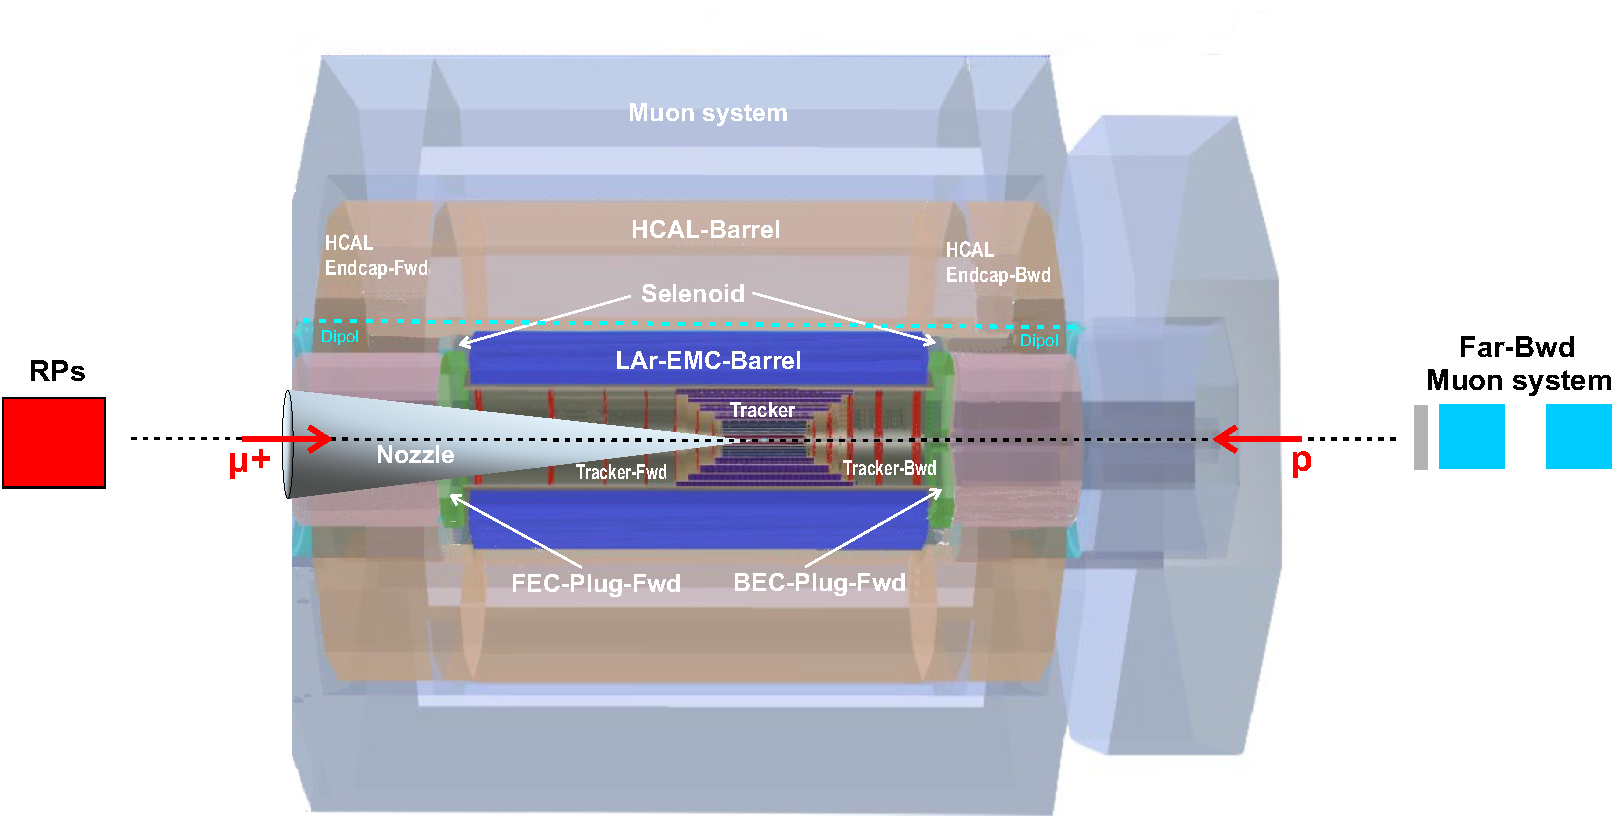
\includegraphics[width=.9\textwidth]{modified_LHeC.pdf}
\caption{Modified LHeC detector for muon-hadron collider.}
\label{fig:modified_LHeC}
\end{figure}

The following changes, such as increased small angle acceptance, background control and mechanical redesign can be implemented preserving the overall LHeC detector architecture.
Small angle physics in the forward direction will be partially lost due to the presence of the nozzle, while the backward acceptance would remain largely preserved. The angle of the nozzle tip should be selected carefully so that it fits well with the beam pipe, final focus magnets, and service lines. Fast timing detectors with precise timing resolution such as LGADs or  PICOSEC-MM should be added to precisely measure the arrival time of particles, allowing the system to distinguish true physics events from delayed background hits. Successful integration requires a joint optimization of the Machine Detector Interface and the timing systems.

\paragraph {\bf Forward Proton Detectors}

While a design and location along the forward beamline suitable for both the LHeC and \lhuc kinematics is preferable in this already highly instrumented region of the accelerator (beam position monitors, beam loss monitors, \ldots), it is subject to a precise study of the beam dynamics in the vicinity of the interaction point, leading to multiple \add{(??)} regions of interest.



\subsubsection{Far Backward Muon Detection}

Additionally, a possibly pre-existing array of Roman Pots in the far forward direction is completed with a Muon System in the far backward direction.
Both are mounted on the beam pipe outside the detector to detect protons and muons with small scattering angles.

With a high-energy incident muon beam, this muon detection in the downstream muon direction (backward) would be essential for DIS measurements and helpful for vector boson fusion processes as well.
Scattering angles can be very small, so detection along the beam line at high pseudorapidity would be required.
For example, DIS scattering with a 1~TeV muon beam leads to muons with $|\eta| \le 7$ for $Q^2\ge  3$~GeV$^2$.
Measuring such TeV muons with a magnet spectrometer is challenging.

One possibility to provide sufficient $\int B\cdot {\rm d}l$ bending is to use the endcap toroid design of the ATLAS experiment \cite{ATLAS:2008xda,ATLAS-Toroid} to instrument several stations along the beamline.
This magnet provides a maximum field of 4.1~T at the innermost radius of 1.05~m (the outer radius is 5.1~m).
Muon detector layers could be placed in front and behind the toroid magnet to measure the bending in the radial direction.
Each magnet could span about 1.6 units of pseudorapidity, so up to 3 stations at ever increasing distance from the collision point would be necessary to fully cover the scattered muon kinematics beyond the central region of the experiment, i.e. $|\eta| \gtrsim 2 $.
This would correspond to stations located roughly 20, 100, and 500~m downstream of the collision point. 

The momentum resolution depends on the precision of the detector technology used. If the achieved detector resolution is of order 150~$\mu$m in front and behind the toroid, then the average momentum resolution (increasing linearly with radius) would be about 5\% at 1~TeV. 

\subsubsection{...}

\subsection{Outlook/next steps}

